\documentclass[aspectratio=169,10pt]{beamer}
\usetheme{Madrid}
\usecolortheme{whale}
\usepackage{booktabs}
\usepackage{graphicx}
\usepackage{amsmath}
\usepackage{colortbl}
\setbeamertemplate{navigation symbols}{}
\setbeamerfont{footnote}{size=\tiny}
\definecolor{mu2eblue}{RGB}{0,51,102}
\setbeamercolor{title}{fg=white}

\title[Shape at Deployed Pitch]{A Stopping Target Optimized at the \emph{Deployed} Foil Pitch}
\subtitle{9D shape search, foil spacing fixed to the baseline design}
\author{Y.\ Oksuzian}
\institute[Mu2e autoresearch]{Mu2e --- autoresearch / closed-loop Bayesian optimization}
\date{2026-08-06}

\begin{document}

\begin{frame}
\titlepage
\end{frame}

% ------------------------------------------------------------------ result
\begin{frame}{Result in one slide}
\begin{block}{}
Hold the foil-to-foil \textbf{gap at the deployed 22.2\,mm} --- so the support and
frame engineering carry over --- and let Bayesian optimization choose everything else.
The result beats the deployed target by \textbf{$+32\%$ S/$\sqrt{B}$} \emph{and} beats the
6D champion on \textbf{both} objectives at once: $+4.9\%$ significance at
\textbf{$-19\%$ detector damage}.
\end{block}
\vspace{0.4em}
\begin{itemize}
  \item \textbf{83 evaluations} (13 transplanted seeds $+$ 70 new), \textbf{zero failures};
        a fourth campaign is running, so the front is still moving.
  \item \textbf{Record} \texttt{foilspfbp03R03\_00}: \textbf{4.30} at
        8.37$\times10^{-7}$ --- vs.\ the deployed target's 3.26 at 6.85$\times10^{-7}$,
        i.e.\ \textbf{$+32\%$ S/$\sqrt{B}$ for $+22\%$ damage}.
  \item It \textbf{strictly dominates} the previous record (\texttt{bp01R00\_03},
        4.29 at 1.23$\times10^{-6}$): same significance, \textbf{32\% less damage},
        a completely different shape.
  \item \textbf{And damage need not be paid at all}: \texttt{bp04R00\_02} reaches
        \textbf{$+19\%$ S/$\sqrt{B}$ at $-13\%$ damage} --- strictly better than the
        deployed target on \emph{both} axes. \textbf{24 of 83} designs do this.
  \item Damage frontier spans \textbf{22$\times$}, floor 5.6$\times10^{-8}$ MeV/POT,
        \textbf{28 Pareto points}.
\end{itemize}
\vspace{0.2em}
\footnotesize
All numbers Run1Bap-scale on the corrected stack (IPA-position fix, strict
zero-overlap preflight).
\end{frame}

% ------------------------------------------------------------------ what we vary
\begin{frame}{What we optimize --- and what we deliberately do not}
\textbf{9-D shape at fixed pitch}: 49 foils generated from $K{=}3$ quadratic control points
for outer radius, half-thickness and hole fraction. \textbf{Extent is pinned} at
$48\times22.222 = \mathbf{1066.7}$~mm --- the deployed foil spacing.
\vspace{0.7em}
\begin{columns}[T]
\begin{column}{0.46\textwidth}
\small
\begin{tabular}{@{}lll@{}}
\toprule
knob & range & \\
\midrule
\texttt{rOut\_\{0,1,2\}} & 50--120 & mm \\
\texttt{hT\_\{0,1,2\}}   & 0.01--0.15 & mm \\
\texttt{f\_\{0,1,2\}}    & 0--0.95 & hole fraction \\
\midrule
\texttt{extent} & \textbf{1066.7} & \textbf{fixed} \\
\bottomrule
\end{tabular}
\end{column}
\begin{column}{0.50\textwidth}
\small
\begin{tabular}{@{}ll@{}}
\toprule
objective & direction \\
\midrule
S/$\sqrt{B}$ (Run1A CE) & \textbf{maximize} \\
detector radiation damage per POT & \textbf{minimize} \\
\bottomrule
\end{tabular}
\end{column}
\end{columns}
\vspace{1em}
\footnotesize
\textbf{Why fix the pitch.} A designed extent scan (10 evaluations, two shapes,
800--2000\,mm) showed S/$\sqrt{B}$ flattening by 1400--1700\,mm: the last 300\,mm buys
$+0.9\%$ significance for $+8\%$ damage. Length is a settled question --- so spend the
search on shape, inside an envelope the hardware already supports.
\end{frame}

% ------------------------------------------------------------------ landscape
\begin{frame}{The landscape}
\begin{center}
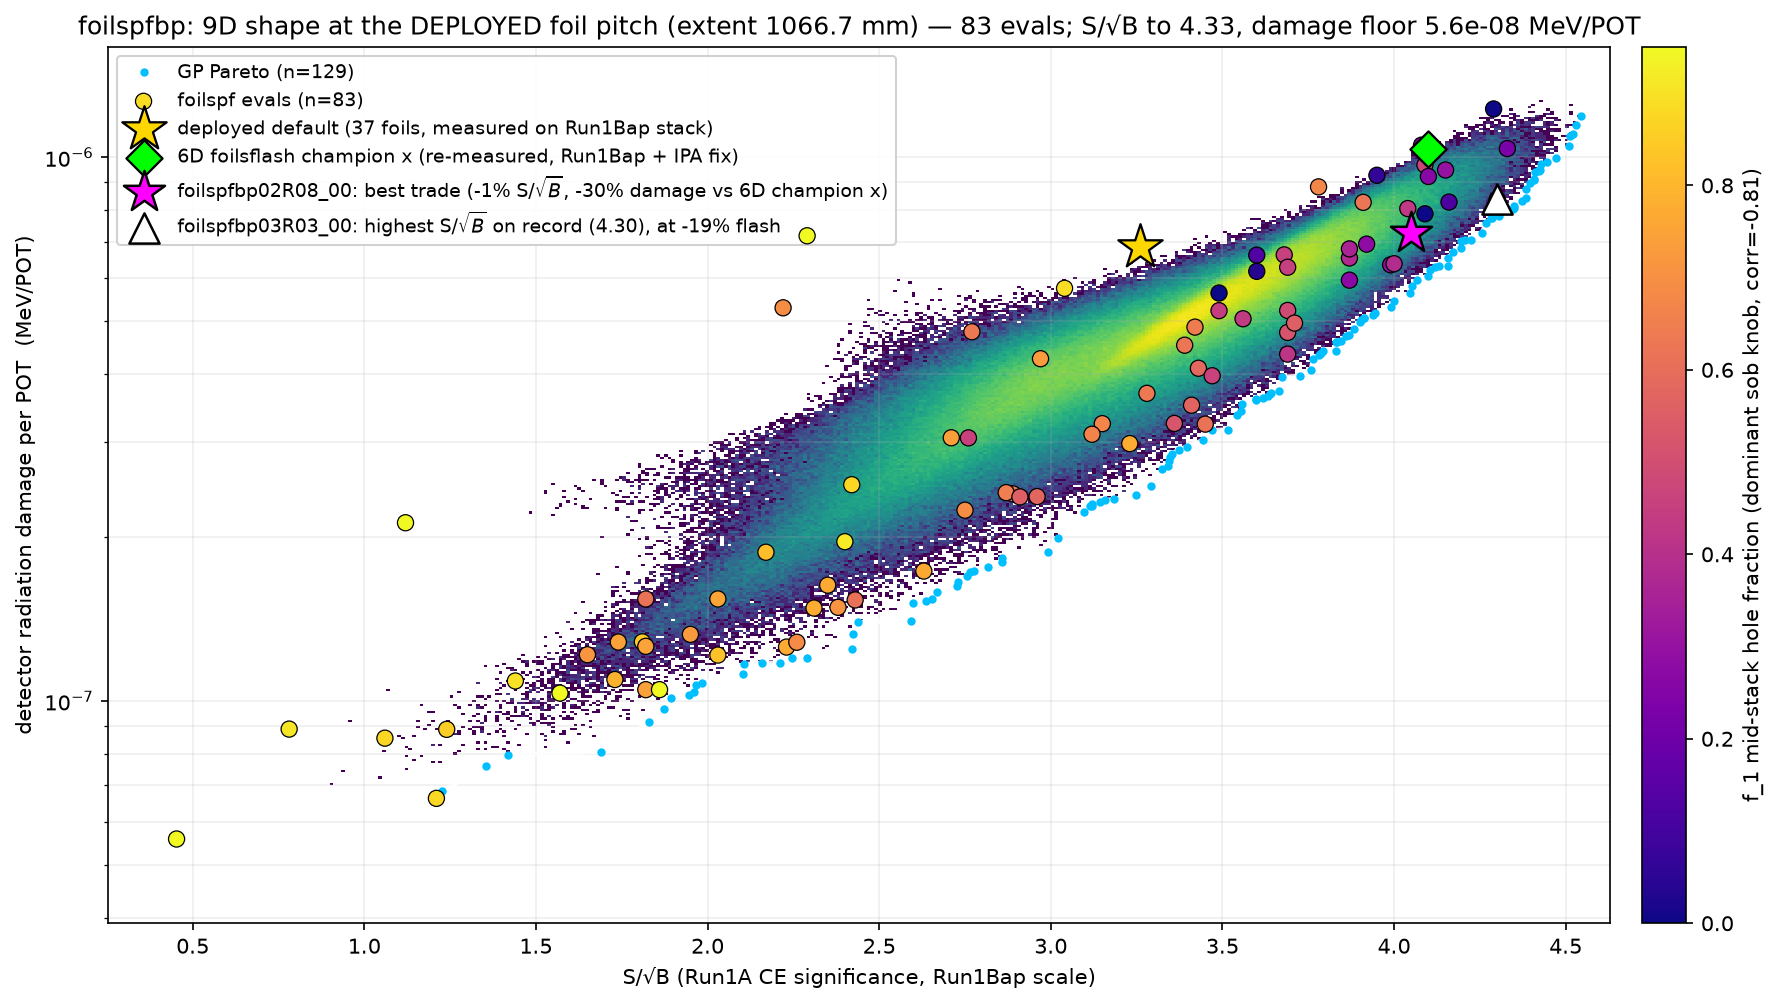
\includegraphics[height=0.66\textheight]{foilspfbp_perpot_cloud.png}
\end{center}
\footnotesize
83 evaluations, GP cloud over the 9D shape box. Gold star $=$ deployed default; green
diamond $=$ the 6D foilsflash champion geometry re-measured on this stack; \textbf{white
triangle} $=$ the record, sitting \emph{to the right of and below} the green diamond ---
better on both axes; magenta star $=$ the lowest-damage point still beating the deployed
target.
Colour $=$ mid-stack hole fraction, the dominant knob (corr $\mathbf{-0.81}$).
\end{frame}

% ------------------------------------------------------------------ anatomy
\begin{frame}{Anatomy of the record}
\begin{columns}
\begin{column}{0.52\textwidth}
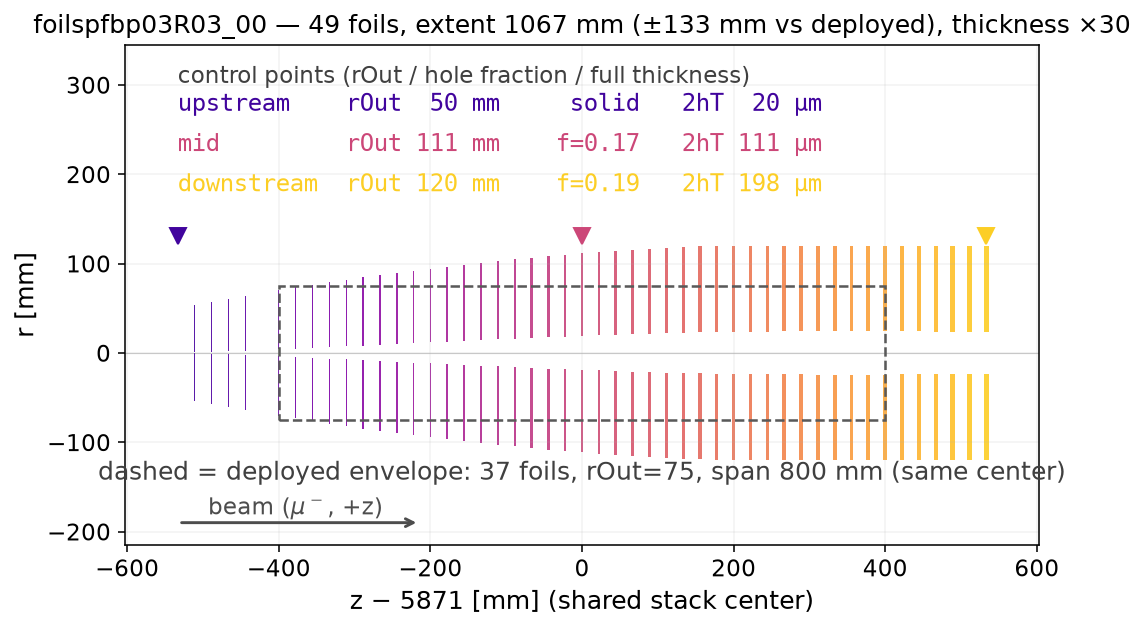
\includegraphics[width=\textwidth]{foilspfbp_bestsob_sketch.png}
\end{column}
\begin{column}{0.46\textwidth}
\small
\begin{tabular}{lcc}
\toprule
design & S/$\sqrt{B}$ & damage \\
\midrule
\texttt{bp03R03\_00} (record)   & \textbf{4.30} & \textbf{0.84} \\
\texttt{bp01R00\_03} (old rec.) & 4.29 & 1.23 \\
\texttt{bp02R03\_00}            & 4.09 & 0.79 \\
\texttt{bp02R08\_00}            & 4.05 & \textbf{0.73} \\
6D champion $x$ (re-meas.)      & 4.10 & 1.04 \\
deployed default                & 3.26 & 0.69 \\
\bottomrule
\end{tabular}
\vspace{0.4em}

{\scriptsize damage in $10^{-6}$ MeV/POT, all on the Run1Bap stack}
\vspace{0.5em}
\begin{itemize}\footnotesize
  \item \textbf{Grows outward, stays nearly solid.} \texttt{rOut} $50 / 111 / 120$\,mm
        with holes almost shut ($f = 0 / 0.17 / 0.19$) --- the reverse of the old record,
        which shrank downstream to \texttt{rOut} 50 and opened an upstream hole.
  \item Thickness ramps $20 \rightarrow 111 \rightarrow 198$\,µm: thin where the beam is
        still intact, thick where it is spent.
  \item Growth is \textbf{symmetric} about the shared centre $z_0 = 5871$: $\pm133$\,mm
        beyond the deployed span, dashed $=$ deployed envelope.
\end{itemize}
\end{column}
\end{columns}
\end{frame}

% ------------------------------------------------------ dominating (damage-neutral)
\begin{frame}{Anatomy of the damage-free point}
\begin{columns}
\begin{column}{0.52\textwidth}
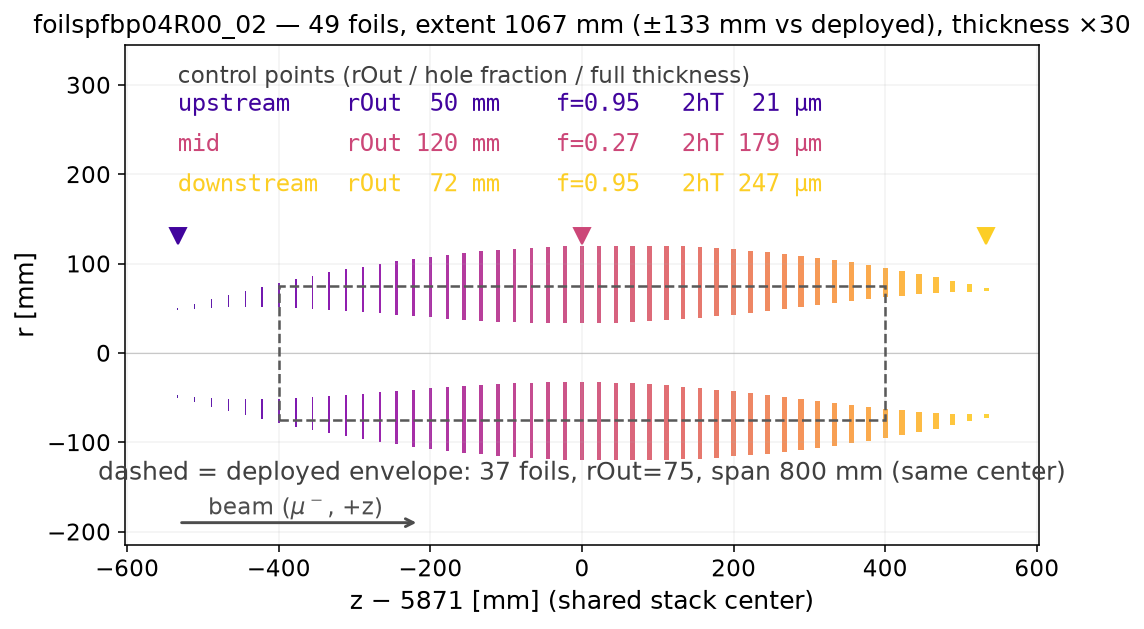
\includegraphics[width=\textwidth]{foilspfbp_domin_sketch.png}
\end{column}
\begin{column}{0.46\textwidth}
\small
\begin{tabular}{lccc}
\toprule
design & S/$\sqrt{B}$ & damage & \\
\midrule
\texttt{bp04R00\_02}    & \textbf{3.87} & \textbf{0.59} & \\
deployed default        & 3.26 & 0.69 & \\
\midrule
\emph{difference}       & \textbf{$+19\%$} & \textbf{$-13\%$} & \\
\bottomrule
\end{tabular}
\vspace{0.4em}

{\scriptsize damage in $10^{-6}$ MeV/POT, Run1Bap stack}
\vspace{0.5em}
\begin{itemize}\footnotesize
  \item \textbf{Better on \emph{both} objectives} than the target we deploy today ---
        no trade at all. \textbf{24 of 83} evaluated designs do this.
  \item \textbf{A wider bore, and one that varies.} The deployed target is already
        annular, but at a \emph{constant} 21.5\,mm hole; this one runs
        \textbf{33--69\,mm} --- 1.5--3$\times$ wider --- and profiles it along $z$.
  \item Carries \textbf{216\,cm$^3$} of aluminium --- $3.4\times$ the deployed
        63\,cm$^3$ --- but only \textbf{1.5\%} of it inside $r<40$\,mm, against the
        deployed target's 22\%.
  \item More stopping mass \emph{and} less flash: the mass moved off the beam axis.
\end{itemize}
\end{column}
\end{columns}
\end{frame}

% ------------------------------------------------------ mid trade (+6% damage)
\begin{frame}{Anatomy of the best point at deployed-level damage}
\begin{columns}
\begin{column}{0.52\textwidth}
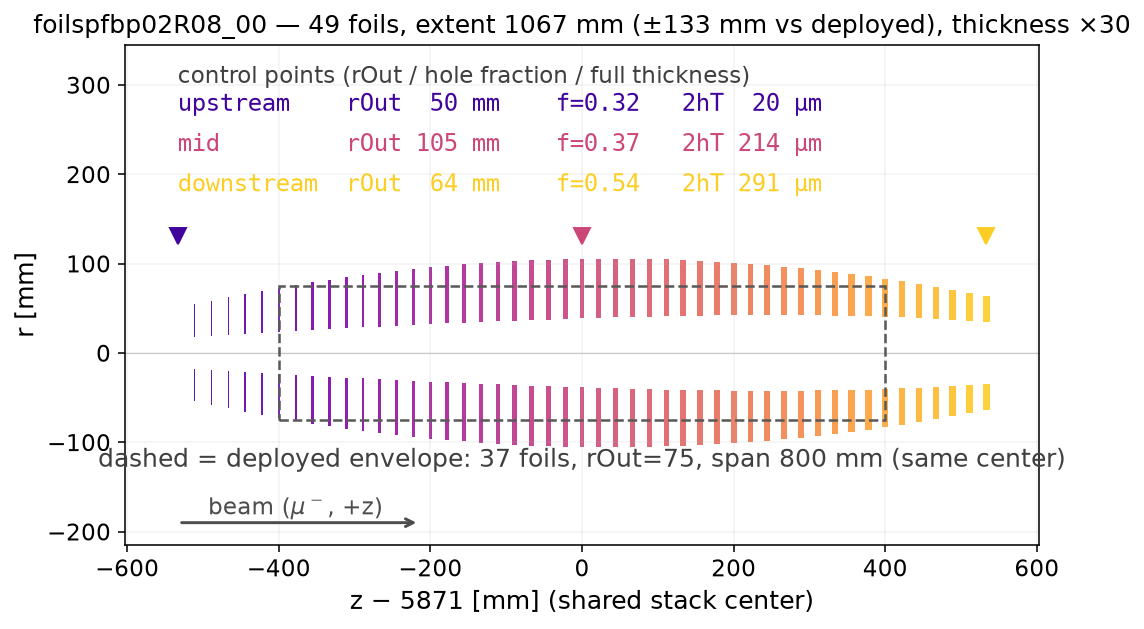
\includegraphics[width=\textwidth]{foilspfbp_midtrade_sketch.png}
\end{column}
\begin{column}{0.46\textwidth}
\small
\begin{tabular}{lcc}
\toprule
design & S/$\sqrt{B}$ & damage \\
\midrule
\texttt{bp02R08\_00}    & \textbf{4.05} & 0.73 \\
deployed default        & 3.26 & 0.69 \\
\midrule
\emph{difference}       & \textbf{$+24\%$} & \textbf{$+6\%$} \\
\bottomrule
\end{tabular}
\vspace{0.4em}

{\scriptsize damage in $10^{-6}$ MeV/POT, Run1Bap stack}
\vspace{0.5em}
\begin{itemize}\footnotesize
  \item \textbf{The most significance available at deployed-level damage}: highest
        S/$\sqrt{B}$ of any design within $10\%$ of the default's flash.
  \item Buys $+5$ points of S/$\sqrt{B}$ over the damage-free design for
        $19$ points of damage --- still only $+6\%$ against today's target.
  \item \textbf{Tighter bore}: 16--42\,mm, straddling the deployed 21.5\,mm, vs the
        damage-free point's 33--69\,mm. Core fraction \textbf{3.1\%} vs 1.5\%.
  \item 212\,cm$^3$ of Al, $3.4\times$ the deployed 63\,cm$^3$, thickest downstream
        (291\,µm) where the beam is spent.
\end{itemize}
\end{column}
\end{columns}
\end{frame}

% ------------------------------------------------------------------ core Al
\begin{frame}{What actually drives the damage --- everything vs.\ the deployed target}
\vspace{-0.2em}
\begin{center}
\scriptsize
\setlength{\tabcolsep}{4pt}
\begin{tabular}{@{}lcccccc@{}}
\toprule
design & S/$\sqrt{B}$ & \textbf{vs default} & damage & \textbf{vs default}
       & Al [cm$^3$] & Al in $r<40$\,mm \\
\midrule
deployed default (37 foils) & 3.26 & --- & 0.69 & --- & 63 & 22.0\% \\
\midrule
\rowcolor{green!12}
\texttt{bp04R00\_02} \textbf{(dominates)} & 3.87 & $\mathbf{+19\%}$ & \textbf{0.59}
                                  & $\mathbf{-13\%}$ & 216 & \textbf{1.5\%} \\
\texttt{bp02R08\_00}              & 4.05 & $+24\%$ & 0.73 & $+6\%$ & 213 & 3.1\% \\
\texttt{bp02R03\_00}              & 4.09 & $+25\%$ & 0.79 & $+15\%$ & 166 & 9.2\% \\
\texttt{bp03R03\_00} (record)     & \textbf{4.30} & $\mathbf{+32\%}$ & 0.84 & $+22\%$ & 206 & 9.6\% \\
\texttt{bp01R00\_03} (old record) & 4.29 & $+32\%$ & 1.23 & $+79\%$ & 153 & 22.0\% \\
\bottomrule
\end{tabular}

{\tiny damage in $10^{-6}$ MeV/POT; all measured on the Run1Bap stack; rows ordered by damage}
\end{center}
\vspace{0.3em}
\begin{columns}[T]
\begin{column}{0.46\textwidth}
\scriptsize
Every optimized design carries \textbf{2.4--3.9$\times$} the default's aluminium --- that is
how it buys the significance. What varies by \textbf{13$\times$} is the damage \emph{penalty}:
$-13\%$ to $+79\%$. It tracks the core column, not the mass column.
\vspace{0.4em}

Over all \textbf{83} evaluated geometries:

\begin{tabular}{@{}lc@{}}
\toprule
Spearman vs.\ damage & $\rho$ \\
\midrule
total Al volume            & $+0.57$ \\
\textbf{Al inside $r<40$\,mm} & $\mathbf{+0.84}$ \\
\bottomrule
\end{tabular}
\end{column}
\begin{column}{0.52\textwidth}
\scriptsize
\begin{itemize}
  \item \texttt{bp01R00\_03} tripled the mass and \emph{kept} the default's 22\% core
        fraction $\rightarrow$ $+79\%$ damage. \texttt{bp04R00\_02} carried \emph{more}
        mass at a 1.5\% core $\rightarrow$ $\mathbf{-13\%}$.
  \item So the lever is \textbf{placement, not mass} --- and it is strong enough that
        \textbf{23 of 81} evaluated designs beat the deployed target on
        \emph{both} objectives at once.
  \item Consistent with Edmonds (DocDB-10898) --- flash parents are central,
        RMS $\approx24$\,mm --- found here by search, not by design.
\end{itemize}
\end{column}
\end{columns}
\end{frame}

% ------------------------------------------------------------------ mechanism
\begin{frame}{Why the optimum moves with the pitch}
\small
The same shape is \emph{not} optimal at every length --- transplanting the 2000\,mm champion
into this envelope leaves performance on the table.
\vspace{0.6em}
\begin{center}
\footnotesize
\begin{tabular}{@{}lcc@{}}
\toprule
shape at 1066--1100\,mm & S/$\sqrt{B}$ & hole profile $f$ \\
\midrule
transplanted 2000\,mm champion (\texttt{SCANA1100}) & 4.16 & 0.43 / 0.12 / \textbf{0.86} \\
optimized at this pitch (\texttt{bp01R00\_03})      & 4.29 & 0.43 / 0 / \textbf{0} \\
\textbf{record} (\texttt{bp03R03\_00})              & \textbf{4.30} & \textbf{0 / 0.17 / 0.19} \\
\bottomrule
\end{tabular}
\end{center}
\vspace{0.6em}
\begin{itemize}
  \item $+3.4\%$ ($\sim$5.6$\sigma$ at $\sigma_{\rm sob}=0.6\%$) purely from re-optimizing the
        shape at fixed length. \textbf{Two independent optima found here both shut the
        downstream hole} the 2000\,mm champion opens wide.
  \item \textbf{Mechanism}: at tight spacing a conversion electron re-crosses more neighbouring
        foils on its way out, so exit-path self-absorption dominates and \emph{open holes stop
        paying}. At 42\,mm pitch the same optimizer opens them wide.
  \item Consistent with the extent scan, where the length gain itself came from the CE
        low-momentum tail retreating --- a narrower signal window against a
        cosmic-dominated background.
\end{itemize}
\end{frame}

% ------------------------------------------------------------------ saturation
\begin{frame}{How fast it converges --- and when to stop}
\small
\begin{center}
\footnotesize
\begin{tabular}{@{}lccl@{}}
\toprule
campaign & evals & best S/$\sqrt{B}$ & outcome \\
\midrule
\texttt{foilspfbp01} & 20 & 3.56 $\rightarrow$ \textbf{4.29} & winner arrived in \textbf{wave 0} \\
\texttt{foilspfbp02} & 20 & 4.29 $\rightarrow$ 4.29 & \textbf{0 of 20} beat it; 7 front points \\
\texttt{foilspfbp03} & 20 & 4.29 $\rightarrow$ \textbf{4.30} & sob \emph{tie} ($0.4\sigma$) at
                                                               \textbf{$-32\%$ damage} \\
\bottomrule
\end{tabular}
\end{center}
\vspace{0.7em}
\begin{itemize}
  \item \textbf{The S/$\sqrt{B}$ ceiling is saturated}: 4.29 $\rightarrow$ 4.30 across 74
        evaluations. Three campaigns of acquisition bought $0.4\sigma$ on that axis.
  \item \textbf{But the front is not.} \texttt{bp03} found the same significance at
        \textbf{32\% less damage} and knocked the old record off the front entirely.
        A repeat campaign never raises the ceiling --- it can still displace the
        champion \emph{by domination}.
  \item Practical rule: stop when the front stops moving, \textbf{not} when the scalar
        record stops moving. Every jump on the sob axis itself came from changing the
        box (extent ceiling, then pitch), never from grinding the same one.
\end{itemize}
\end{frame}

% ------------------------------------------------------------------ next
\begin{frame}{Conclusion \& next steps}
\small
\begin{itemize}
  \item A target optimized \textbf{at the deployed foil pitch} gives $+32\%$ S/$\sqrt{B}$
        over the deployed design, inside an envelope the existing support structure was
        built for.
  \vspace{0.4em}
  \item \textbf{No trade needed at the top any more.} The record beats the 6D champion on
        \emph{both} objectives ($+4.9\%$ S/$\sqrt{B}$, $-19\%$ damage). Against the
        \emph{deployed} target it is $+32\%$ S/$\sqrt{B}$ for $+22\%$ damage.
  \vspace{0.4em}
  \item \textbf{A no-cost option exists.} \texttt{bp04R00\_02}: $+19\%$ S/$\sqrt{B}$ at
        $\mathbf{-13\%}$ damage --- strictly better than the deployed target on both
        objectives, at the deployed foil pitch. This is the point to take to full
        simulation first.
  \vspace{0.4em}
  \item \textbf{Needed --- prove it with full simulation.} Every number here is a fast score
        (S/$\sqrt{B}$ and damage extracted without full reconstruction). The best configs must
        go through the full \texttt{dig} $\rightarrow$ \texttt{mcs} $\rightarrow$ \texttt{nts}
        chain before this is an $R_{\mu e}$ claim.
  \vspace{0.4em}
  \item \textbf{Regime caveat.} Run-1a is cosmic-dominated, so part of the gain is
        window-economics. Shape gains (stopping $\times$ acceptance) survive any background
        model; length gains do not.
  \vspace{0.4em}
  \item \textbf{Design lever, transferable}: damage tracks \emph{core} aluminium
        ($\rho = +0.84$), not total ($+0.57$) --- keep the mass, move it off the axis.
        \textbf{Search closed}: \texttt{foilspfbp} at 93 evals; a wider-box successor
        (\texttt{foilspfbw}, 20 evals) did not improve on it at the deployed damage budget.
\end{itemize}
\end{frame}

\end{document}
